%%%%%%%%%%%%%%%%%%%%%%%%%%%%%%%%%%%%%%%%%
% Beamer Presentation
% LaTeX Template
% Version 1.0 (10/11/12)
%
% This template has been downloaded from:
% http://www.LaTeXTemplates.com
%
% License:
% CC BY-NC-SA 3.0 (http://creativecommons.org/licenses/by-nc-sa/3.0/)
%
%%%%%%%%%%%%%%%%%%%%%%%%%%%%%%%%%%%%%%%%%

%----------------------------------------------------------------------------------------
%	PACKAGES AND THEMES
%----------------------------------------------------------------------------------------

\documentclass{beamer}

\mode<presentation> {

% The Beamer class comes with a number of default slide themes
% which change the colors and layouts of slides. Below this is a list
% of all the themes, uncomment each in turn to see what they look like.

%\usetheme{default}
%\usetheme{AnnArbor}
%\usetheme{Antibes}
%\usetheme{Bergen}
%\usetheme{Berkeley}
%\usetheme{Berlin}
%\usetheme{Boadilla}
%\usetheme{CambridgeUS}
%\usetheme{Copenhagen}
%\usetheme{Darmstadt}
%\usetheme{Dresden}
%\usetheme{Frankfurt}
%\usetheme{Goettingen}
%\usetheme{Hannover}
%\usetheme{Ilmenau}
%\usetheme{JuanLesPins}
%\usetheme{Luebeck}
\usetheme{Madrid}
%\usetheme{Malmoe}
%\usetheme{Marburg}
%\usetheme{Montpellier}
%\usetheme{PaloAlto}
%\usetheme{Pittsburgh}
%\usetheme{Rochester}
%\usetheme{Singapore}
%\usetheme{Szeged}
%\usetheme{Warsaw}

% As well as themes, the Beamer class has a number of color themes
% for any slide theme. Uncomment each of these in turn to see how it
% changes the colors of your current slide theme.

%\usecolortheme{albatross}
%\usecolortheme{beaver}
%\usecolortheme{beetle}
%\usecolortheme{crane}
%\usecolortheme{dolphin}
%\usecolortheme{dove}
%\usecolortheme{fly}
%\usecolortheme{lily}
%\usecolortheme{orchid}
%\usecolortheme{rose}
%\usecolortheme{seagull}
%\usecolortheme{seahorse}
%\usecolortheme{whale}
%\usecolortheme{wolverine}

%\setbeamertemplate{footline} % To remove the footer line in all slides uncomment this line
\setbeamertemplate{footline}[page number] % To replace the footer line in all slides with a simple slide count uncomment this line

\setbeamertemplate{navigation symbols}{} % To remove the navigation symbols from the bottom of all slides uncomment this line
}

\usepackage{graphicx} % Allows including images
\usepackage{booktabs} % Allows the use of \toprule, \midrule and \bottomrule in tables
%\usepackage {tikz}
\usepackage{tkz-graph}
\usepackage{hyperref}
\usepackage{ulem}
\hypersetup{
    colorlinks=true,
    linkcolor=blue,
    filecolor=magenta,
    urlcolor=cyan,
}
\GraphInit[vstyle = Shade]
\tikzset{
  LabelStyle/.style = { rectangle, rounded corners, draw,
                        minimum width = 2em, fill = yellow!50,
                        text = red, font = \bfseries },
  VertexStyle/.append style = { inner sep=5pt,
                                font = \normalsize\bfseries},
  EdgeStyle/.append style = {->, bend left} }
\usetikzlibrary {positioning}

%\usepackage {xcolor}
\definecolor {processblue}{cmyk}{0.96,0,0,0}
%----------------------------------------------------------------------------------------
%	TITLE PAGE
%----------------------------------------------------------------------------------------

\title[Short title]{Piezoelectric effect measurement update (Noise and initial design considerations)} % The short title appears at the bottom of every slide, the full title is only on the title page

\author{Ari Pedersen, Danny Vander-Hyde} % Your name
\institute[Syracuse University] % Your institution as it will appear on the bottom of every slide, may be shorthand to save space
{
Syracuse University\\ % Your institution for the title page
\medskip
}
\date{June 21, 2019} % Date, can be changed to a custom date

\begin{document}

\begin{frame}
\titlepage % Print the title page as the first slide
\end{frame}

\begin{frame}
\frametitle{Overview} % Table of contents slide, comment this block out to remove it
\tableofcontents % Throughout your presentation, if you choose to use \section{} and \subsection{} commands, these will automatically be printed on this slide as an overview of your presentation
\end{frame}

%----------------------------------------------------------------------------------------
%	PRESENTATION SLIDES
%----------------------------------------------------------------------------------------

%------------------------------------------------
\section{How big is the Piezoelectric effect?}
\begin{frame}{Some preliminary figures}
\begin{itemize}
  \item According to Marty Fejer $\frac{\partial \phi}{\partial \mathrm{E}} \approx 4.5*10^{-10} \frac{\mathrm{m}}{\mathrm{V}}$
  \item Conservatively we can attempt to create a setup that would generate Electric fields on the order of 10 V / 2.5 cm = \sout{400} \textcolor{red}{40} V/m \textcolor{red}{(Apparently I can't math)}
  \item Could also up the voltage and decrease the distance to get a larger effect
  \item This would lead to an effect of $1.8*10^{-8} \; [\mathrm{rad}]$ or $3.05*10^{-14} [\mathrm{m}]$
  \item This is for a single layer so we could multiply by the number of AlGaAs layers? (Maybe increases the effect by an order of magnitude?)
\end{itemize}
\end{frame}

\section{Competing with laser frequency noise}
\begin{frame}{Light source: Mephisto 2000 NE}
 \begin{figure}[H]
  \centering
  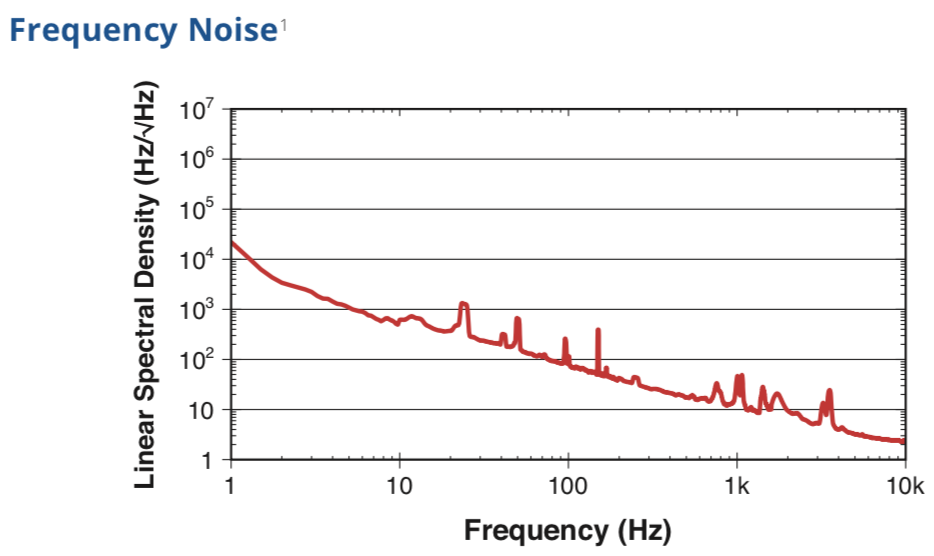
\includegraphics[width=90mm]{freq_noise_mephisto_2000NE.png}
 \end{figure}
\end{frame}

\begin{frame}{Frequency noise to phase noise}
\begin{itemize}
  \item Assuming that the largest laser frequency fluctuations ($\Delta f_\mathrm{laser}$) 11,500 Hz away from the carrier frequency. Can calculate this as phase noise $\big(\frac{\Delta f_{\mathrm{laser}}}{f_{\mathrm{laser}}}\big)$ on the order of $4.08*10^{-11}\; [\mathrm{rad}]$
  \item If we are to use a simple Fabry-Perot cavity to measure this effect, we would need:
$$\frac{\Delta f_{\mathrm{laser}}}{f_{\mathrm{laser}}}< \frac{\Delta L_{\mathrm{cav}}}{L_{\mathrm{cav}}}$$
Where I am considering $\Delta L_{\mathrm{cav}}$ to be the induced length change due to the piezoelectric effect.
  \item Assuming we have a 10 cm length cavity we can estimate $\frac{3.05*10^{-14}}{.01} = 3.05*10^{-12}\; [\mathrm{rad}]$ which lies an order of magnitude below the effect we wish to measure. :(
  \item Can modulate the electric field at some higher frequency where the frequency noise is less of an issue (how fast can we modulate the field and still notice the effect? $\rightarrow$ Impulse / Step response analysis)
\end{itemize}
\end{frame}

\begin{frame}{Frequency noise to phase noise \textcolor{red}{Stefan notes}}
\begin{itemize}
  \item Stefan mentioned that up to 10kHz you can assume that Piezo-electric response of the coating is flat up to 10kHz
  \item If we are to use a simple Fabry-Perot cavity to measure this effect, we would need:
$$\frac{\Delta f_{\mathrm{laser}}}{f_{\mathrm{laser}}}< \frac{\Delta L_{\mathrm{cav}}}{L_{\mathrm{cav}}}$$
Where I am considering $\Delta L_{\mathrm{cav}}$ to be the induced length change due to the piezoelectric effect.
  \item Assuming we have a 10 cm length cavity we can estimate $\frac{3.05*10^{-14}}{.01} = 3.05*10^{-12}\; [\mathrm{rad}]$ which lies an order of magnitude below the effect we wish to measure. :(
  \item Can modulate the electric field at some higher frequency where the frequency noise is less of an issue (how fast can we modulate the field and still notice the effect? $\rightarrow$ Impulse / Step response analysis)
\end{itemize}

\end{frame}

\begin{frame}{PDH locking}

\begin{itemize}
  \item First attempt to suppress laser frequency noise while keeping simple cavity design in mind.
  \item Black states (\href{https://youtu.be/tX884B8GrEE}{ref}) that a closed loop PDH system can suppress frequency noise ($n$) below the reference cavity pole frequency by a factor of $$\frac{1}{1 + H(s)*D(s)*K(s)}$$
Where H(s) [Hz/V] is the laser transfer function, D(s) [V/Hz] is the PDH transfer function, and K(s) is the servo gain.
  \item Don’t have exact values to propose but this could be a place to start.
  \item Propose we use the LIGO PMC we have on the AMM table as refrence cavity. (Might want to double check how destructive this could be to phase camera peeps)
  \item If this does not provide enough suppression, we might have to move on to an interferometer design.

\end{itemize}
\end{frame}

\section{Electrode / Sample mount}
\begin{frame}{Electrode design}
\begin{itemize}
  \item Am thinking of machining a thin square aluminum plate significantly larger than the size of the optic so to avoid field fringe effects. (Might need to do some quick calculations to establish the minimum size of this plate)
  \item Will also want to drill a hole in the center of the plate so to allow the beam to pass through to the AlGaAs sample without introducing any spatial defects to the intra-cavity beam. (Can do some calculations for optimal aperture size)
\end{itemize}
\end{frame}

\begin{frame}{Sample / electrode mount(s)}
  \item Traditional metallic optic mounts could introduce unwanted charge distributions. Need to think of ways around this. Here are some inital thoughts:
\\~\\
\textbf{In-air}
\begin{itemize}
    \item 3D printed flexure optic mount
    \item Could potentially be a simple one piece print
\end{itemize}
\\~\\
\textbf{In-vacuum}
\begin{itemize}
    \item Monolithic fused silica holder (Work on 3d printed concept? request to have made at Corning?)
    \item Don’t know how we would embed a fused silica holder in vacuum (suspended?) (clamped on table?)
\end{itemize}
\end{frame}

\end{document}
